%!TEX TS-program = xelatex

% Официальный шаблон презентации НИУ ВШЭ в beamer (LaTeX)
% Версия 2.0
% Язык — русский

\documentclass[aspectratio=169]{beamer}

\newbool{russian}
\booltrue{russian}
\usepackage{HSE-theme/beamerthemeHSE}

%%% Работа с русским языком и шрифтами
\usepackage{multirow}
\usepackage{listings} 
\usepackage[dvipsnames,table]{xcolor}
\usepackage[english,russian,shorthands=off]{babel}
\usepackage[no-math]{fontspec}
\usepackage{makecell}
	\IfFontExistsTF{HSE Sans}
		{\newcommand{\presentationfont}{HSE Sans}}
		{\newcommand{\presentationfont}{Arial}}
	\setsansfont{\presentationfont}
	\setmonofont{Courier New}
\usepackage[most]{tcolorbox}

\usepackage{mathspec}
	\setmathsfont(Digits,Latin,Greek)[Numbers={Lining,Proportional}]{\presentationfont}
	\setmathrm[Numbers={Lining,Proportional}]{\presentationfont}
\uselanguage{russian}
\languagepath{russian}
\deftranslation[to=russian]{Theorem}{Теорема}
\deftranslation[to=russian]{Definition}{Определение}
\deftranslation[to=russian]{Definitions}{Определения}
\deftranslation[to=russian]{Corollary}{Следствие}
\deftranslation[to=russian]{Fact}{Факт}
\deftranslation[to=russian]{Example}{Пример}
\deftranslation[to=russian]{Examples}{Примеры}

\usepackage{booktabs}
\usepackage{array}
\graphicspath{{images/}}


\newcommand{\term}[1]{{\textcolor{HSEblue}{#1}}}
\newcommand{\cmd}[1]{\textcolor{HSEblue}{\texttt{#1}}}
\lstset{ 
    basicstyle=\color{HSEblue}\ttfamily\small,
    numbers=left,
    numberstyle=\color{HSEblue}\ttfamily\scriptsize,
    frame=single,
    columns=fullflexible,
    keepspaces=true,
    showstringspaces=false,
    breaklines=true,
    rulecolor=\color{HSEblue},
}


%% Информация об авторе и выступлении

\title[Мобильные колесные роботы]{Основы автономной навигации. Знакомство с Nav2}
\subtitle{Проектный семинар <<Мобильные колесные роботы>>}
\author[Команда курса]{Дергачев Степан  Алексеевич, \texttt{\href{mailto:sadergachev@hse.ru}{sadergachev@hse.ru}} \\ Муравьев Кирилл Федорович, \texttt{\href{mailto:kmuravev@hse.ru}{kmuravev@hse.ru}}}
\institute{Факультет компьютерных наук НИУ ВШЭ}
\date{26 ноября 2026}


% Отключаем активные кавычки babel для совместимости с mathspec.
\AtBeginDocument{\shorthandoff{"}}
% Убираем лишний пробел после полноширинного блока номера страницы.
% Внешний вид и файл темы HSE остаются прежними.
\makeatletter
\patchcmd{\beamer@@tmpl@footline}{\end{beamercolorbox} }{\end{beamercolorbox}}{}{}
\makeatother
% Подпись под иллюстрацией ведёт на страницу, где опубликован оригинал.
\newcommand{\figsource}[2]{\par\smallskip{\centering\footnotesize\href{#1}{#2}\par}}
\begin{document}
\frame[plain]{\titlepage}

\section{Задача навигации} % 14 минут, включая титульный слайд

\begin{frame}{Задача автономной навигации}
\begin{columns}[c,onlytextwidth]
\column{.55\textwidth}
\begin{itemize}
\item Робот должен переместиться из начального состояния $s = (p_{x,s},p_{x,s}, \theta_s)$ в заданное целевое $g = (p_{x,g},p_{y,g}, \theta_g)$, избегая столкновений с препятствиями.
\item Связанные задачи:
\begin{itemize}
  \normalsize
  \item Обход последовательности точек
  \item Покрытие области
\end{itemize}
\end{itemize}
\column{.41\textwidth}
\centering
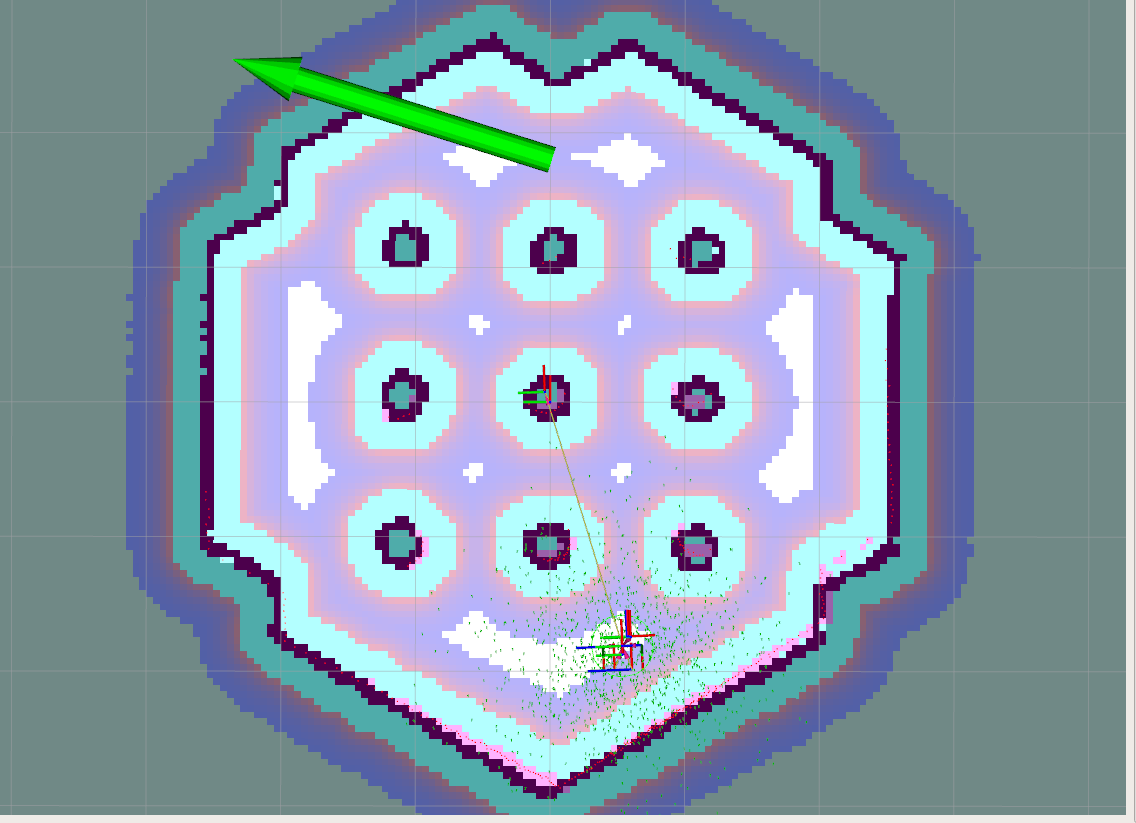
\includegraphics[width=\linewidth]{rviz_goal.png}
\end{columns}
\end{frame}

\begin{frame}{Автономная навигация в широком смысле}

\renewcommand{\arraystretch}{1.2}
% \small
\begin{tabular}{>{\raggedright\arraybackslash}m{0.23\textwidth}>{\raggedright\arraybackslash}m{0.68\textwidth}}
\toprule
\term{Задача} & \term{В чем суть} \\
\midrule

Картирование & По измерениям датчиков строится представление среды \\
Локализация & По карте и измерениям датчиков оценивается состояние робота \\
Планирование & По карте и оценке позы строится путь к цели (и/или последовательность управлений) \\
Исполнение & Контроллер робота переводит управления в сигналы актуаторам робота\\
\bottomrule
\end{tabular}
\vfill

\end{frame}


\begin{frame}{Автономная навигация в широком смысле}

\renewcommand{\arraystretch}{1.2}
% \small
\begin{tabular}{>{\raggedright\arraybackslash}m{0.23\textwidth}>{\raggedright\arraybackslash}m{0.68\textwidth}}
\toprule
\term{Задача} & \term{В чем суть} \\
\midrule

Картирование & По измерениям датчиков строится представление среды \\
Локализация & По карте и измерениям датчиков оценивается состояние робота \\
\rowcolor{HSEblue!15}Планирование & По карте и оценке позы строится путь к цели (и/или последовательность управлений) \\
Исполнение & Контроллер робота переводит управления в сигналы актуаторам робота\\
\bottomrule
\end{tabular}
\vfill

\end{frame}

\begin{frame}{Глобальное и локальное планирование}
\begin{columns}[T,onlytextwidth]
\column{.48\textwidth}
\begin{block}{Глобальный уровень}
  \begin{itemize}
    \item Ищет путь от текущего состояния до целевого
  \end{itemize}

\end{block}
\column{.48\textwidth}
\begin{block}{Локальный уровень}
    \begin{itemize}
    \item Ведет робота вдоль глобального пути, избегая столкновений
  \end{itemize}
\end{block}
\end{columns}
\end{frame}

\begin{frame}{Глобальное планирование}
\begin{columns}[c,onlytextwidth]
\small
\column{.54\textwidth}
\begin{block}{Цели:}
  \begin{itemize}
    \item Найти глобальный маршрут
    \item Проверить достижимость
  \end{itemize}
\end{block}
\begin{block}{Особенности:}
  \begin{itemize}
    \item Большой горизонт планирования
    \item Низкая (относительно) частота запуска
    \item Геометрический путь (без управлений)
    \item (Обычно) не учитывает форму робота и его кино-динамические ограничения
  \end{itemize}
\end{block}
\column{.35\textwidth}
\centering
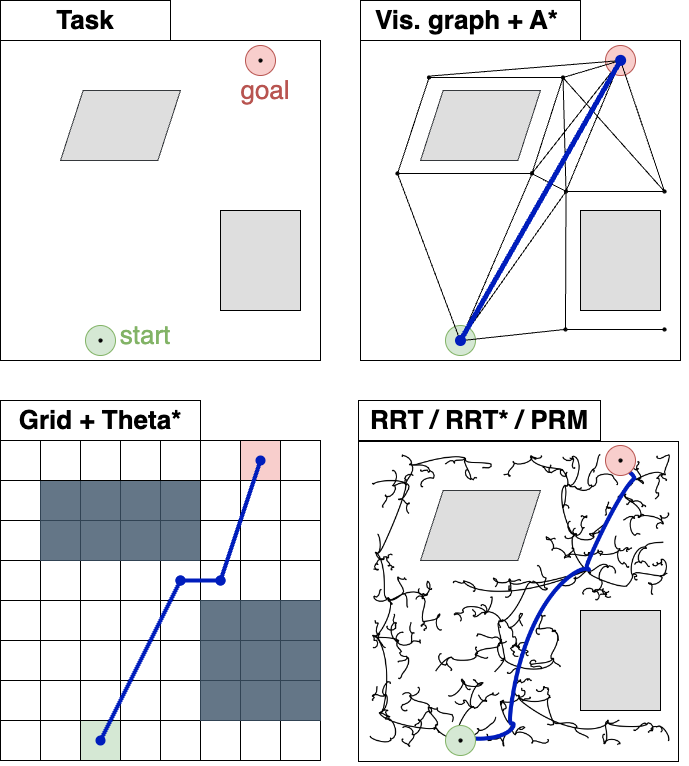
\includegraphics[width=\linewidth]{glob_plan.png}
\end{columns}
\end{frame}

\begin{frame}{Локальное планирование}
\begin{columns}[c,onlytextwidth]
\small
\column{.59\textwidth}
\begin{block}{Цели:}
  \begin{itemize}
    \item Найти управление для следования траектории
    \item Избежать столкновений с динамическими препятствиями
  \end{itemize}
\end{block}
\begin{block}{Особенности:}
  \begin{itemize}
    \item Маленький горизонт планирования
    \item Высокая частота запуска
    \item Текущее управляющее воздействие / последовательность воздействий
    \item Зачастую учитывает форму и ограничения робота
  \end{itemize}
\end{block}
\column{.40\textwidth}
\centering
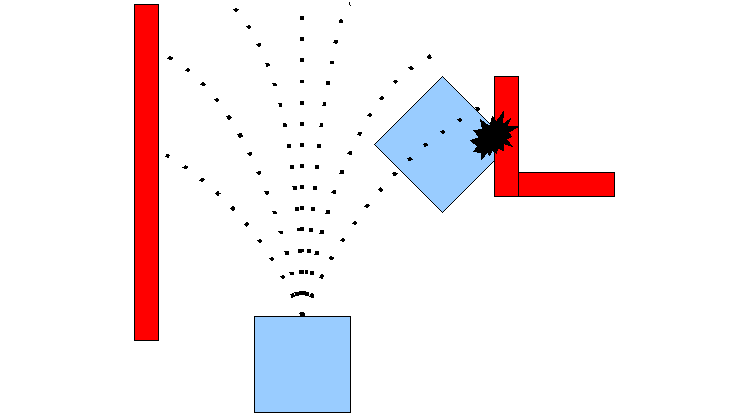
\includegraphics[width=\linewidth]{dwa.png}
\end{columns}
\end{frame}

\section{Архитектура Nav2} % 12 минут

\begin{frame}{Архитектура Nav2}
\centering
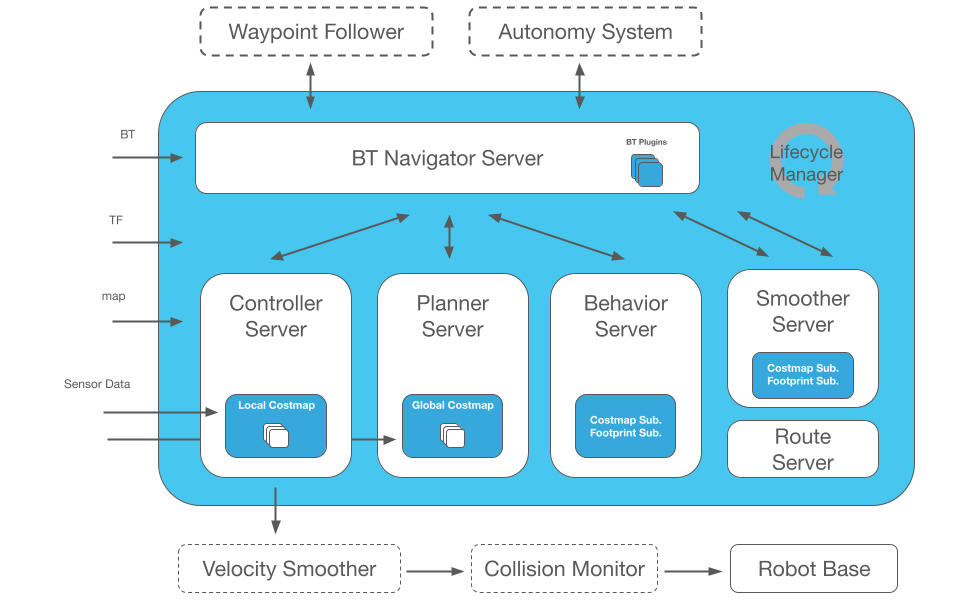
\includegraphics[width=0.7\linewidth]{nav2_architecture.png}
\end{frame}

\begin{frame}{Что не является частью Nav2}
\begin{itemize}
  \item \term{Картирование$^*$.} Может использовать карту от внешнего источника
  \item \term{Локализация$^*$}. Использует позицию и скорость, полученные из дерева \cmd{tf2} и топика \cmd{odom}. Ожидается существование следующего преобразования:
  \begin{center}
    \cmd{map} $\to$ \cmd{odom} $\to$ \cmd{base\_link}
  \end{center}
  \item \term{Исполнение}. Команы в формате \cmd{cmd\_vel} отправляются на исполнение драйвером робота (например через \cmd{ros2\_control})
  \end{itemize}
  \noindent\rule{\textwidth}{0.4pt}\smallskip
  \footnotesize
  \begin{itemize}
    \item[$^*$] \textit{Nav2 содержит в себе пакеты \cmd{map\_server} и \cmd{amcl}. При работе с готовой картой узел \cmd{map\_server} публикует её, а \cmd{amcl} оценивает состояние. Также поддерживается родственный проект \cmd{slam\_toolbox}, реализующий одновременное картирование и локализацию}
  \end{itemize}
\end{frame}

\begin{frame}{Planner Server}
Принимает целевую позу через Action-интерфейс \cmd{/compute\_path\_to\_pose} (инициируется при получении сообщения из топика \cmd{/goal\_pose}) и публикует рассчитанный глобальный путь типа \cmd{nav\_msgs/Path} в топик \cmd{/plan}.
\begin{block}{Варианты планировщиков}
\begin{itemize}
  \item \term{NavFn} -- быстрый поиск пути по сетке (на основе Дейкстры / A*) для роботов с круглой базой.
  \item \term{Smac} -- поиск пути с учетом радиуса поворота и габаритов робота.
  \item \term{Theta Star} -- поиск пути, строящий спрямленные траектории.
\end{itemize}
\end{block}
\end{frame}

% \begin{frame}{Controller Server}
% Сервер получает путь через \cmd{FollowPath}. На каждом шаге управления плагин вычисляет команду скорости по пути, текущей позе, скорости и локальной карте стоимости.
% \begin{itemize}
%   \item Regulated Pure Pursuit выбирает опорную точку на пути и снижает скорость на крутых поворотах.
%   \item DWB проверяет несколько вариантов движения на коротком интервале и оценивает их по близости к пути и препятствиям.
% \end{itemize}
% \medskip
% Сервер отдельно проверяет продвижение робота и достижение цели с заданным допуском по положению и углу.
% \end{frame}

% \begin{frame}{Rotation Shim Controller}
% У дифференциального робота начальное направление пути может сильно отличаться от ориентации корпуса. Например, путь идёт вдоль коридора, а робот стоит поперёк.
% \medskip
% \begin{enumerate}
%   \item При получении пути Rotation Shim сравнивает направление его начального участка с курсом робота.
%   \item Если угол больше порога, контроллер задаёт поворот на месте.
%   \item После разворота команды вычисляет основной контроллер, указанный в параметре \cmd{primary\_controller}.
% \end{enumerate}
% \end{frame}

% \section{Представление среды в Nav2} % 13 минут

% \begin{frame}{Карта стоимости (costmap)}
% \begin{columns}[c,onlytextwidth]
% \column{.49\textwidth}
% Карта занятости хранит сведения о свободных и занятых участках среды. В карте стоимости каждая клетка получает значение, которое планировщик или контроллер использует при оценке движения.
% \medskip

% На рисунке красные клетки заняты. Синим показана область, в которой центр робота будет слишком близко к препятствию. Красный контур в центре~--- проекция корпуса (\cmd{footprint}).
% \column{.47\textwidth}
% \centering
% 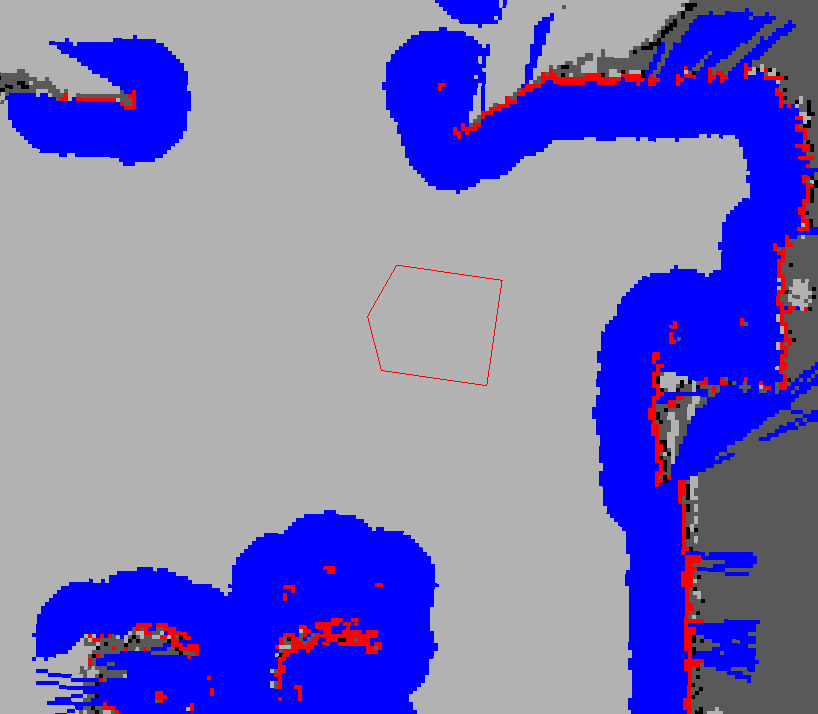
\includegraphics[width=\linewidth,height=5.65cm,keepaspectratio]{costmap_rviz.png}
% \figsource{https://ftp.osuosl.org/pub/ros/ros_wiki_mirror/costmap_2d.html}{Карта стоимости в RViz. ROS Wiki, costmap\_2d}
% \end{columns}
% \end{frame}

% \begin{frame}{Слои карты стоимости}
% \begin{description}[Obstacle Layer]
%   \item[Static Layer] Переносит в сетку данные карты занятости, например стены помещения.
%   \item[Obstacle Layer] Отмечает препятствия по сканам лидара или облаку точек. Если луч лидара проходит через ранее занятую клетку, отметку можно снять.
%   \item[Inflation Layer] Повышает стоимость клеток в окрестности отмеченных препятствий.
% \end{description}
% \medskip
% Слои обновляют одну сетку в порядке, заданном в конфигурации. Inflation Layer обычно стоит последним в списке.
% \end{frame}

% \begin{frame}{Инфляция препятствий}
% \begin{columns}[c,onlytextwidth]
% \column{.31\textwidth}
% \small
% По горизонтали отложено расстояние от центра робота до ближайшей занятой клетки, по вертикали~--- стоимость.
% \medskip

% В пределах вписанного радиуса корпус задевает препятствие при любом повороте. Дальше стоимость убывает до границы, заданной \cmd{inflation\_radius}.
% \column{.67\textwidth}
% \centering
% 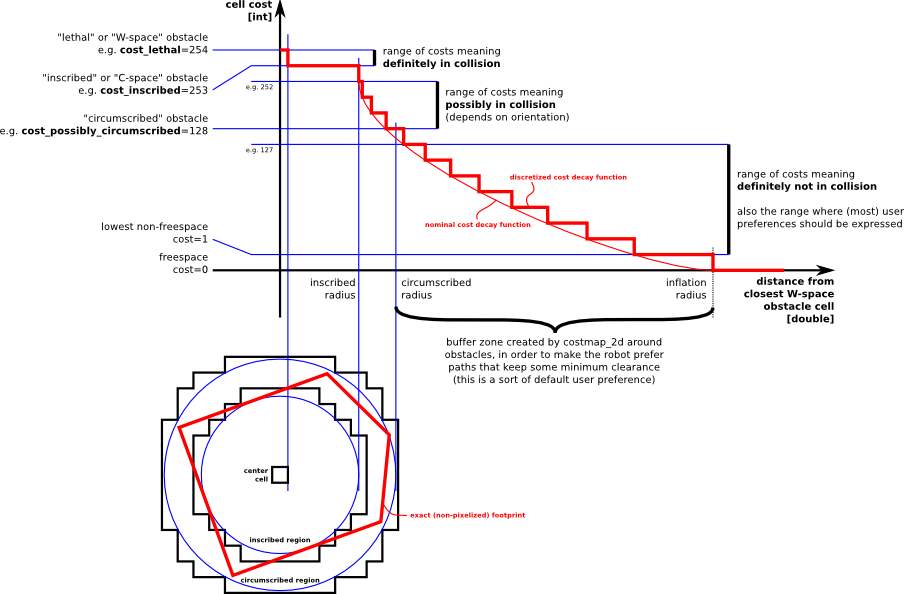
\includegraphics[width=\linewidth,height=6.05cm,keepaspectratio]{costmap_inflation.png}
% \figsource{https://ftp.osuosl.org/pub/ros/ros_wiki_mirror/costmap_2d.html}{Зависимость стоимости от расстояния. ROS Wiki, costmap\_2d}
% \end{columns}
% \end{frame}

% \begin{frame}{Глобальная и локальная карты стоимости}
% \small
% \centering
% \renewcommand{\arraystretch}{1.42}
% \begin{tabular}{@{}>{\raggedright\arraybackslash}p{2.6cm}>{\raggedright\arraybackslash}p{4.8cm}>{\raggedright\arraybackslash}p{4.9cm}@{}}
% \toprule
%  & \textbf{Глобальная карта} & \textbf{Локальная карта} \\
% \midrule
% Сервер & Planner Server & Controller Server \\
% Область & Обычно вся карта помещения & Окно, которое движется вместе с роботом \\
% Координаты & Обычно \cmd{map} & Обычно \cmd{odom} \\
% Источники & Карта занятости, при необходимости данные датчиков & В первую очередь данные бортовых датчиков \\
% \bottomrule
% \end{tabular}
% \par\medskip
% У каждой карты свои разрешение, частота обновления и список слоёв.
% \end{frame}

% \section{Выполнение задачи} % 16 минут

% \begin{frame}[fragile]{Жизненный цикл узлов Nav2}
% После запуска процесса сервер находится в состоянии \cmd{unconfigured}. Lifecycle Manager последовательно выполняет два перехода.
% \begin{description}[configure]
%   \item[configure] Сервер читает параметры, загружает плагины и переходит в состояние \cmd{inactive}.
%   \item[activate] Сервер переходит в \cmd{active} и начинает принимать задачи.
% \end{description}
% Порядок запуска узлов задаётся в параметрах Lifecycle Manager. Команда для проверки состояния сервера
% \begin{lstlisting}[numbers=none]
% ros2 lifecycle get /planner_server
% \end{lstlisting}
% \end{frame}

% \begin{frame}{BT Navigator}
% Клиент передаёт целевую позу через действие ROS~2 \cmd{NavigateToPose}. Для движения через несколько поз предусмотрено \cmd{NavigateThroughPoses}.
% \medskip

% Для выбранной задачи BT Navigator запускает дерево поведения. В нём задан порядок вызовов серверов и условия для повторного планирования или восстановления после ошибки.
% \medskip

% Во время движения клиент получает обратную связь и может отменить задачу.
% \end{frame}

% \begin{frame}{Дерево поведения (Behavior Tree)}
% При каждом обходе дерева управляющий узел обращается к дочерним узлам. Статус действия показывает, продолжается ли оно (\cmd{RUNNING}), завершилось успешно (\cmd{SUCCESS}) или с ошибкой (\cmd{FAILURE}).
% \begin{itemize}
%   \item \cmd{Sequence} выполняет дочерние узлы по порядку. Если один из них вернул ошибку, последовательность прерывается.
%   \item \cmd{Fallback} при ошибке переходит к следующему варианту и останавливается при первом успехе.
% \end{itemize}
% \end{frame}

% \begin{frame}{Перепланирование во время движения}
% \centering
% 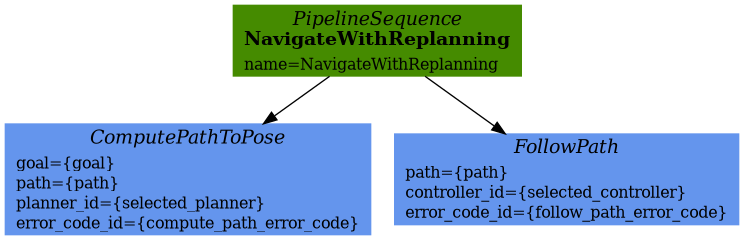
\includegraphics[width=.80\textwidth,height=3.85cm,keepaspectratio]{navigation_subtree.png}
% \figsource{https://docs.nav2.org/jazzy/getting_started/nav2_behavior_trees/detailed_behavior_tree_walkthrough/detailed_behavior_tree_walkthrough/}{Фрагмент дерева навигации без ветвей восстановления. Nav2}
% \medskip
% \raggedright
% \cmd{PipelineSequence} позволяет снова вызвать планировщик, пока контроллер выполняет \cmd{FollowPath}. В типовом дереве Jazzy планировщик вызывается примерно раз в секунду.
% \end{frame}

% \begin{frame}{Восстановление после ошибки (recovery)}
% В типовом дереве Nav2 при ошибке планирования можно очистить глобальную карту стоимости и повторить поиск. Для ошибки следования пути предусмотрена очистка локальной карты. Видимое лидару препятствие при следующем обновлении появится снова.
% \medskip

% Доступны также действия Behavior Server.
% \begin{itemize}
%   \item \cmd{Spin}~--- повернуться на месте.
%   \item \cmd{Wait}~--- подождать, например пока освободится проход.
%   \item \cmd{BackUp}~--- отъехать назад.
% \end{itemize}
% Число повторных попыток ограничено. Если они исчерпаны, клиент получает сообщение о неудаче.
% \end{frame}

% \begin{frame}{Обработка запроса NavigateToPose}
% \begin{enumerate}
%   \item BT Navigator принимает цель и передаёт её в дерево поведения.
%   \item Узел \cmd{ComputePathToPose} запрашивает путь у Planner Server. Путь сохраняется в общей памяти дерева (\textit{blackboard}).
%   \item Узел \cmd{FollowPath} читает путь и передаёт его в Controller Server. Контроллер выдаёт команды скорости до достижения цели или ошибки.
%   \item Когда контроллер сообщает о достижении цели, дерево завершается успешно. При ошибке дерево выбирает ветвь восстановления или завершает задачу с ошибкой.
% \end{enumerate}
% \end{frame}

% \section{Компоненты, запуск и настройка} % 15 минут

% \begin{frame}{Дополнительные серверы Nav2}
% \begin{description}[Smoother Server]
%   \item[Smoother Server] Сглаживает путь, например убирает мелкие изломы после поиска по сетке.
%   \item[Route Server] Строит маршрут по заданному графу. Рёбра графа могут соответствовать проездам между стеллажами.
%   \item[Docking Server] Управляет подъездом к док-станции и стыковкой. Так робот может самостоятельно подъехать к зарядным контактам.
% \end{description}
% \end{frame}

% \begin{frame}{Обработка команд скорости}
% \begin{block}{Velocity Smoother}
% Получает команды контроллера и ограничивает скорость и ускорение. Например, при ступенчатом изменении заданной скорости база разгоняется постепенно.
% \end{block}
% \begin{block}{Collision Monitor}
% Проверяет заданные зоны вокруг корпуса по данным датчиков. При появлении препятствия в зоне может ограничить скорость или остановить робота.
% \end{block}
% Если используются оба узла, Collision Monitor ставят после Velocity Smoother, перед контроллером базы.
% \end{frame}

% \begin{frame}[fragile]{Запуск отдельных узлов}
% Запуск Planner Server со штатным файлом параметров Jazzy
% \begin{lstlisting}[numbers=none]
% bringup=$(ros2 pkg prefix --share nav2_bringup)
% ros2 run nav2_planner planner_server --ros-args \
%   --params-file "$bringup/params/nav2_params.yaml"
% \end{lstlisting}
% В собственном launch-файле указывают нужные серверы, пути к параметрам и переназначения топиков. Список управляемых узлов передают в Lifecycle Manager.
% \end{frame}

% \begin{frame}[fragile]{Запуск nav2\_bringup}
% Запуск с картой из пакета курса и временем симулятора
% \begin{lstlisting}[numbers=none]
% maps="$(ros2 pkg prefix --share example_webots_localization)/maps"
% ros2 launch nav2_bringup bringup_launch.py \
%   map:="$maps/three_boxes.yaml" use_sim_time:=true
% \end{lstlisting}
% \begin{itemize}
%   \item Робот уже публикует сканы, одометрию и TF. Launch-файл запускает локализацию по карте и навигационные серверы.
%   \item Параметры конкретного робота передают через \cmd{params\_file}. В них указывают размеры корпуса, системы координат и топики датчиков. Начальную позу для AMCL можно задать в RViz.
% \end{itemize}
% \end{frame}

% \begin{frame}{Файлы конфигурации Nav2}
% \begin{description}[Параметры узлов]
%   \item[Launch-файл] Перечень узлов, передаваемые им параметры и переназначения топиков.
%   \item[Описание карты] YAML-файл с путём к изображению, размером клетки в метрах и положением сетки в системе координат карты.
%   \item[Параметры узлов] YAML-файл с разделом для каждого узла. В нём задают частоты, источники данных, размеры карт стоимости и имена плагинов.
%   \item[Дерево поведения] XML-файл с узлами дерева и связями между ними. Путь к файлу задают в параметрах BT Navigator.
% \end{description}
% \end{frame}

% \begin{frame}[fragile]{Плагины Nav2}
% Планировщики, контроллеры и слои карт стоимости подключаются как плагины. В этом примере сервер загружает один планировщик.
% \begin{lstlisting}[numbers=none]
% planner_server:
%   ros__parameters:
%     planner_plugins: ["GridBased"]
%     GridBased:
%       plugin: "nav2_navfn_planner::NavfnPlanner"
%       use_astar: false
% \end{lstlisting}
% \small
% В поле \cmd{planner\_id} запроса указывают имя \cmd{GridBased}. Сервер выбирает по нему плагин NavFn. При \cmd{use\_astar: false} он использует алгоритм Дейкстры.
% \end{frame}

% \begin{frame}{Пример настройки двух карт стоимости}
% В дверном проёме стоит коробка. Робот остановился перед ней, а новый глобальный путь снова проходит через дверь.
% \begin{columns}[T,onlytextwidth]
% \column{.47\textwidth}
% \begin{block}{Глобальная карта}
% Подключены Static Layer и Inflation Layer. На сохранённой карте дверь свободна.
% \end{block}
% \column{.47\textwidth}
% \begin{block}{Локальная карта}
% Obstacle Layer получает сканы лидара. Контроллер видит занятые клетки в дверном проёме.
% \end{block}
% \end{columns}
% \medskip
% Если добавить в глобальную карту слой наблюдений лидара, при следующем планировании можно учесть коробку и искать путь через другую дверь.
% \end{frame}

% \begin{frame}{Материалы}
% \begin{itemize}
%   \item \href{https://docs.nav2.org/jazzy/getting_started/navigation_concepts/}{Nav2 Jazzy. Компоненты навигационной системы}.
%   \item \href{https://ftp.osuosl.org/pub/ros/ros_wiki_mirror/costmap_2d.html}{ROS Wiki. Карта стоимости и инфляция препятствий в costmap\_2d}.
%   \item \href{https://docs.nav2.org/jazzy/getting_started/nav2_behavior_trees/detailed_behavior_tree_walkthrough/detailed_behavior_tree_walkthrough/}{Nav2 Jazzy. Дерево навигации с перепланированием и восстановлением}.
%   \item \href{https://github.com/ros-navigation/navigation2/blob/jazzy/nav2_bringup/params/nav2_params.yaml}{Файл параметров nav2\_params.yaml} и \href{https://github.com/ros-navigation/navigation2/blob/jazzy/nav2_bringup/launch/bringup_launch.py}{bringup\_launch.py} из пакета nav2\_bringup.
% \end{itemize}
% \end{frame}
\end{document}
